%========================================= Kapitola: Astrofyzika =============================================
\chapter{Úvod}
\minitoc
\newpage
  \wikiAstrofyzika  je vědní obor ležící na rozhraní \emph{fyziky} a \emph{astronomie}. Zabývá se fyzikou 
  vesmíru, včetně fyzikálních vlastností (svítivost, hustota, teplota, chemické složení) astronomických 
  objektů jako jsou hvězdy, galaxie a mezihvězdná hmota, jakož i jejich vzájemné působení.
  
  Podle metod výzkumu těchto objektů se dělí na \emph{fotometrii}, \emph{spektroskopii},
  \emph{radioastronomii}, \emph{astrofyziku rentgenovou}, \emph{infračervenou}, \emph{ultrafialovou} a 
  \emph{neutrinovou}. Každý z těchto podoborů se dále dělí na praktickou a teoretickou část. Praktická 
  získává potřebná data. Teoretická s pomocí fyzikálních zákonů vysvětluje pozorované cho\-vá\-ní vesmírných 
  těles.
  
  \section{Historie astrofyziky}
  
  \section{Základní vztahy}
    \begin{itemize}
      \item \wikiAU - \emph{astronomická jednotka}: průměrná vzdálenost Země od Slunce, $150\cdot10^6\ km$. 
      Vzájemné vzdálenosti planet či jiných objektů sluneční soustavy vy\-já\-dře\-né v AU poskytují 
      relativně názorné měřítko vzdáleností těchto objektů od sebe. Přesná hodnota je $$1 AU = 149\ 597\ 870\ 
      691 \pm 6\ m$$ Kvůli vyšší přesnosti \emph{Mezinárodní astronomická unie} (International Astronomical 
      Union, IAU) přijala novou de\-fi\-ni\-ci, podle které je AU délka poloměru nerušené oběžné kruhové 
      dráhy tělesa se zanedbatelnou hmotností, pohybujícího se okolo Slunce rychlostí $0,017\ 202\ 098\ 950$ 
      radiánů za den ($86\ 400\ s$). 
        \begin{itemize}
          \item Vzdálenost Země od Slunce je $1,00 ± 0,02\ AU$.
          \item Měsíc obíhá kolem Země ve vzdálenosti $0,0026 \pm 0,0001\ AU$.
          \item Mars je od Slunce vzdálen $1,52 \pm 0,14 AU$.
          \item Jupiter je od Slunce vzdálen $5,20 \pm 0,05\ AU$.
          \item Nejvzdálenější člověkem vyrobené těleso, sonda Voyager 1, bylo 31. prosince 2007 ve    
                vzdálenosti $104,93\ AU$ od Slunce.
          \item Průměr sluneční soustavy bez \emph{Oortova oblaku} je přibližně $105\ AU$.
          \item Průměr sluneční soustavy s Oortovým oblakem se odhaduje na $50\ 000$ až $100\ 000\ AU$.
          \item Nejbližší hvězda (po Slunci), Proxima Centauri, se nachází přibližně ve vzdálenosti 
                $268\ 000\ AU$.
          \item Průměr hvězdy Betelgeuze je $2,57\ AU$.
          \item Vzdálenost Slunce od středu Galaxie je přibližně $1,7\cdot10^9\ AU$.
          \item Velikost viditelného vesmíru je asi $8,66\cdot10^{14}\ AU$.
        \end{itemize}
      \item \textbf{l.y.} - \emph{světelný rok}: vzdálenost, kterou světlo ulétna za jeden rok, 
            $9,46\cdot10^{12}\ km$,
      \item \textbf{pc} - \emph{parsek, paralaktická sekunda}: vzdálenost, ze které by poloměr oběžné dráhy   
            Země byl kolmo k zornému paprsku vidět pod úhlem $1''$, $30,9\cdot10^{12}$ km. 
    \end{itemize}
    
    \begin{example} 
      Spočtěte, jakou vzdálenost v metrech vyjadřuje jeden parsek \protect\cite[s.~3]{Kulhanek2009}.
      
      \textbf{řešení}: $1\ pc$ (paralaktická sekunda) je vzdálenost, ze které vidíme velkou poloosu oběžné 
      dráhy Země kolem Slunce pod uhlem $\varphi = 1''$. Úhel $1''$ je tak malý, že strany $VS$ a $VZ$ na 
      obrázku prakticky splývají a místo pravého trojúhelníka $VSZ$ můžeme použít definiční vztah úhlu v 
      obloukové míře (\emph{velkost úhlu je možné určit jako poměr délky oblouku vymezeného rameny na 
      kružnici opsané kolem vrcholu k poloměru této kružnice}). Proto $$\varphi = \frac{R_{SZ}}{l} 
      \rightarrow l = \frac{R_{SZ}}{\varphi},$$ 

      \begin{figure}[ht!]
          \centering
          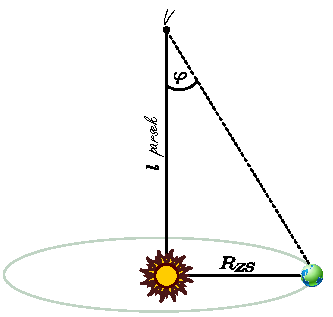
\includegraphics[width=0.8\linewidth]{ex_parsek.pdf}
          \caption[Parsek]{Parsek}
          \label{afyz:fig_ex_parsek}
      \end{figure}
      
      kde $l$ je vzdálenost $1\ pc$ v metrech, $R_{SZ}$ je vzdálenost země od Slunkce a $\varphi$ je úhel jedné vteřiny vyjádřený v radiánech. 
      $$l = \frac{1,5\cdot10^{11}\ m}{\frac{1}{60\cdot60}\cdot\frac{2\pi}{360}}\cong 3\cdot10^{16}\ m.$$  
      
    \end{example}
    
   Další jednotkou, kterou se v astrofyzice měří vzdálenost dvou vesmírných těles, je \emph{paralaxa}. 
   Pozorovací místa musí být od sebe výrazně vzdálena, aby například při měření vzdálenosti naší nejbližší 
   hvězdy - \emph{Proxima Centauri} byla paralaxa vůbec měřitelná. Vzdálenost této hvězdy je 4,2 světelných 
   let (nebo 270 000 AU) od Země.
   
    \begin{example}
      Najděte paralaxu Proximy Centauri, která je od nás vzdálená asi 4,2 světelného roku \protect\cite[s.~4]{Kulhanek2009}.
      
      \begin{figure}[ht!]
          \centering
          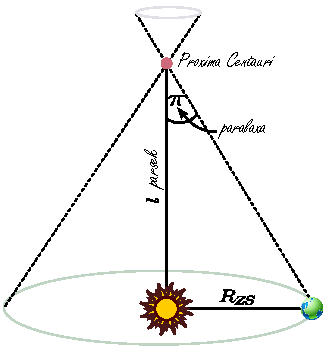
\includegraphics[width=\linewidth]{ex_Proxima_Centauri_paralaxa.pdf}
          \caption[Paralaxa naší nejbližší hvězdy]{Paralaxa naší nejbližší hvězdy}
          \label{afyz:fig_ex_paralaxa}
      \end{figure}
            
      \textbf{Řešení}: Díky pohybu Země kolem Slunce se zdá, že blízké hvězdy opisují oproti vzdáleným 
      elipsu. Úhlový poloměr této elipsy se nazývá paralaxa hvězdy. Lze ji změřit jen pro nejbližší hvězdy. Z 
      definice úhlu (jako v předchozím příkladě) tedy vyplývá, že
      $$\pi = \frac{R_{ZS}}{l} = \frac{1,5\cdot10^{11}\ m}{4,2 l.y} = \frac{1,5\cdot10^{11}\ 
      m}{4,2\cdot9,5\cdot10^{15}\ m}	\cong 3,7\cdot10^{-6}\ rad,$$ což je přibližně $0.76''$. Vidíme, že i u 
      druhé nejbližší hvězdy po Slunci není paralaxa ani celá $1''$.
    \end{example}

\printbibliography[heading=subbibliography]